\chapter{A MACHINE LEARNING BASED APPROACH TO QUANTIFYING NOISE IN MEDICAL IMAGES}
\label{chap:SPIE1}

\let\thefootnote\relax\footnotetext{
Parts of this chapter previously appeared as:
A. Chowdhury, K.~S. Aggour, S.~M. Gustafson, B. Yener,
``A Machine Learning Approach to Quantifying Noise in Medical Images.''
\emph{Medical Imaging 2016: Digital Pathology},
vol. 9791, pp. 979110U, 2016.}

%%% INTRODUCTION
\section{Introduction}

As advances in medical imaging technology are resulting in significant growth of biomedical image data, new techniques are needed to automate the process of identifying images of low quality. Automation is needed because it is very time consuming for a domain expert such as a medical practitioner or a biologist to manually separate good images from bad ones. While there are plenty of de-noising algorithms in the literature, their focus is on designing filters which are necessary but not sufficient for determining how useful an image is to a domain expert.
Thus a computational tool is needed to assign a score to each image based on its perceived quality. In this paper, we introduce a machine learning-based score and call it the Quality of Image (QoI) score. The QoI score is defined based on the probabilities of classification using the logistic regression classifier.
We test our technique on clinical image data obtained from cancerous tissue samples. We used 723 tissue samples that are stained by three different markers (abbreviated as CK15, pck26, E\_cad) leading to a total of 2,169 images. The results show a distribution of the QoI for each of the three markers that correspond to the actual quality of the images from the marker. Our automated labeling is in agreement with the domain experts with an F1-score of 0.9044 on average . Furthermore, images maybe recovered based on a probability threshold and forwarded for further post-processing.

%%% Data
\section{Data}

The data we use is in the form of microscopic images. The colon cohort in this analysis was collected from the Clearview Cancer Institute of Huntsville Alabama from 1993 until 2002, with 747 patient tumor samples collected as formalin-fixed paraffin-embedded specimens. The median follow-up time of patients in this cohort is 4.1 years, with a maximum of over ten years. Stage 2 patients comprise 38 \% of this cohort, stage 1 and 2 combined are 65 \% of the total patients. We have stained and processed 747 CRC subjects described above on tissue microarrays for 63 target proteins of consequence to cancer biology and ancillary image processing and analysis. A full description of materials and methods was described recently in \cite{gerdes2013highly}.
The images are stained with four different markers. The markers are Ecadherin (E\_cad), pan-Keratin (pck26), Keratin15 (CK15) and Vimentin. The first three markers stain epithelial cells in the tissue, while Vimentin stains mesenchymal cells - a complementary set of cells in the image obtained from the same tissue sample, as shown in Fig. 1. The raw dataset consists of 747 tissue samples and each tissue sample has four images from each marker; resulting in a total of 2,988 images. Since images with the Vimentin marker provides complementary information to the other three markers; we do not use this marker for our analysis and prediction. We do, however, perform preliminary noise reduction on all four markers. The images marked with E\_cad have the least amount of noise associated with them. Images stained with pck26 and CK15 have more noise and undesirable artifacts in them. 723 images from the 747 samples were selected by the pathologist for this work.

\begin{figure}
    \centering
    \begin{subfigure}[b]{0.3\textwidth}
        \centering
        \includegraphics[width=\textwidth]{img/SPIE/ecad_example.eps}
        \caption{E\_cad}
        \label{fig:ecad_example}
    \end{subfigure}
    \hfill
    \begin{subfigure}[b]{0.3\textwidth}
        \centering
        \includegraphics[width=\textwidth]{img/SPIE/pck26_example.eps}
        \caption{pck26}
        \label{fig:pck26_example}
    \end{subfigure}
    \hfill
    \begin{subfigure}[b]{0.3\textwidth}
        \centering
        \includegraphics[width=\textwidth]{img/SPIE/CK15_example.eps}
        \caption{CK15}
        \label{fig:CK15_example}
    \end{subfigure}
    \caption{Examples of a single colon tumor tissue sample stained with three different markers}
    \label{fig:example_images}
\end{figure}

\subsection{Feature extraction}

We quantify the information in the three markers (E\_cad, pck26, CK15) by texture features. Texture based features maybe used as a way to quantify the amount of signal or noise in an image.  These set of 13 features are based on gray-level intensity values, and texture information \cite{haralick1979statistical, haralick1973textural} in the images. 
In addition to the features, labels are assigned to each image by domain experts based on the amount of noise in them. The label +1 is assigned if the image has some signal in it. This class is colloquially referred to as the \textit{good} class.  Images with a lot of noise in them where there is almost no signal are labelled as -1 or the \textit{bad} class.


\subsection{Data preprocessing}
The three markers (CK15, pck26, E\_cad, and combined) corresponding to each tissue sample are combined together to provide us with 723 x 3 = 2169 samples. We perform 5-fold cross validation on this data to compute the quality of image score and report the accuracy and F1-score on the validation data.
The data is highly imbalanced. The ratio of bad to good images is roughly 1 : 18. Therefore, it is important to try to redress this imbalance. We use the synthetic minority oversampling technique (SMOTE) \cite{chawla2002smote} on this data to perform oversampling. 
Principal components analysis (PCA) \cite{world1987principal} is performed to reduce the number of features from 13 such that it captures 95 \% of the information. This reduces the number of dimensions to 5.


\section{Methods and experiments}
In this section, we describe the methods that we used in our analysis of the images and also show the results that we achieved from the application of these methods on our data.

\subsection{Random undersampling}
The data in the two classes is imbalanced because the number of images in the \textit{good} class (images with high amount of signal) far outnumbers the number of instances in the \textit{bad} or noisy class. The ratio of imbalance is approximately 1:30. We perform random undersampling to redress the imbalance and ensure that the sizes of the two classes (good and bad) are the same.

\subsection{Classification and analysis}
We used the logistic regression classification algorithm for performing classification. The F1-score for classification is 0.9044 ($\pm$  0.03 standard deviation). We use the F1-score instead of accuracy as the classification metric because of the imbalance in the dataset.

\subsection{Quality of image score}
The \textit{Quality of Image (QoI)} score is defined as the probability that an image is from the \textit{good} class. It is given by Eq. \ref{eq:1}.
\begin{equation}
\begin{gathered} 
S_i \ =  \ p_{i1} 
\end{gathered}
\label{eq:1}
\end{equation}
A high value of the probability indicates that the image has high quality and must be used for analysis. A low value of the probability denotes that the image belongs to the \textit{bad} class and it can be discarded. An intermediate value of the probability is interesting because it denotes there is some signal in the image and that it maybe used for analysis. We denote such an image to be \textit{ugly} which is neither \textit{good} nor \textit{bad}.
 The three sample images in the following figure show examples \textit{good}, \textit{bad} and \textit{ugly} classes according to the QoI score. 

\begin{figure} [ht!]
    \centering
    \begin{subfigure}[b]{0.3\textwidth}
        \centering
        \includegraphics[width=\textwidth]{img/SPIE/E_cad_AFRemoved_260143_9945.eps}
        \caption{A \textit{good} image from E\_cad marker with a \textit{QoI} of 0.9945}
        \label{fig:ecad_example}
    \end{subfigure}
    \hfill
    \begin{subfigure}[b]{0.3\textwidth}
        \centering
        \includegraphics[width=\textwidth]{img/SPIE/CK15_AFRemoved_269_084_0077.eps}
        \caption{A \textit{bad} image from CK15 marker with a \textit{QoI} of 0.0077}
        \label{fig:pck26_example}
    \end{subfigure}
    \hfill
    \begin{subfigure}[b]{0.3\textwidth}
        \centering
        \includegraphics[width=\textwidth]{img/SPIE/pck26_AFRemoved_260_084_5262.eps}
        \caption{A \textit{ugly} image from pck26 marker with a \textit{QoI} of 0.5262}
        \label{fig:CK15_example}
    \end{subfigure}
    \caption{Examples of \textit{good}, \textit{bad} and \textit{ugly} images based on the \textit{QoI} score.}
    \label{fig:example_images}
\end{figure}


\subsection{Defining the \textit{ugly} class}
In addition to the good and bad class, we observe that there exist some images, which have both quantities of signal and noise in relatively equal proportion. Classifying this kind of image as good or bad becomes very subjective. Therefore, it seems intuitive to define a third class, referred to as the ugly class. We define and extract this class based on the QoI scores in the following manner.
We plot histograms of these discrete distributions as shown in Fig. \ref{fig:ugly_distributions}. We can clearly see from the distributions that the scores form three distinct clusters. Therefore, we performed K-means clustering on the normalized score values with K=3. The cluster of images corresponding to the scores in the middle range is termed the ugly class. Images in the ugly class require further (possibly manual) processing. Thus, we are most interested in the images that are near the middle range, the images that we can recover. 
We threshold out the ugly images with the help of the middle cluster in K-means and using a threshold for scores. The thresholds are taken to be between 0.3 to 0.6. We have found that 7.22 \%, 9.77 \% and 29.30 \% of images in E\_cad, pck26 and CK15 respectively, lie in this middle cluster. The results are intuitive because the amount of noise increases progressively from E\_cad to CK15 to pck26. A number of things may be done with the images that belong to the ugly class. They may be forwarded to medical practitioners for inspection. Further noise elimination may also be performed, or as we have done, the ?combined? image could be used as a proxy for the images belonging to this ugly class. This is because the ?combined? image best captures the important information in the images stained with the three different markers.

 \begin{figure}[H]
\centering
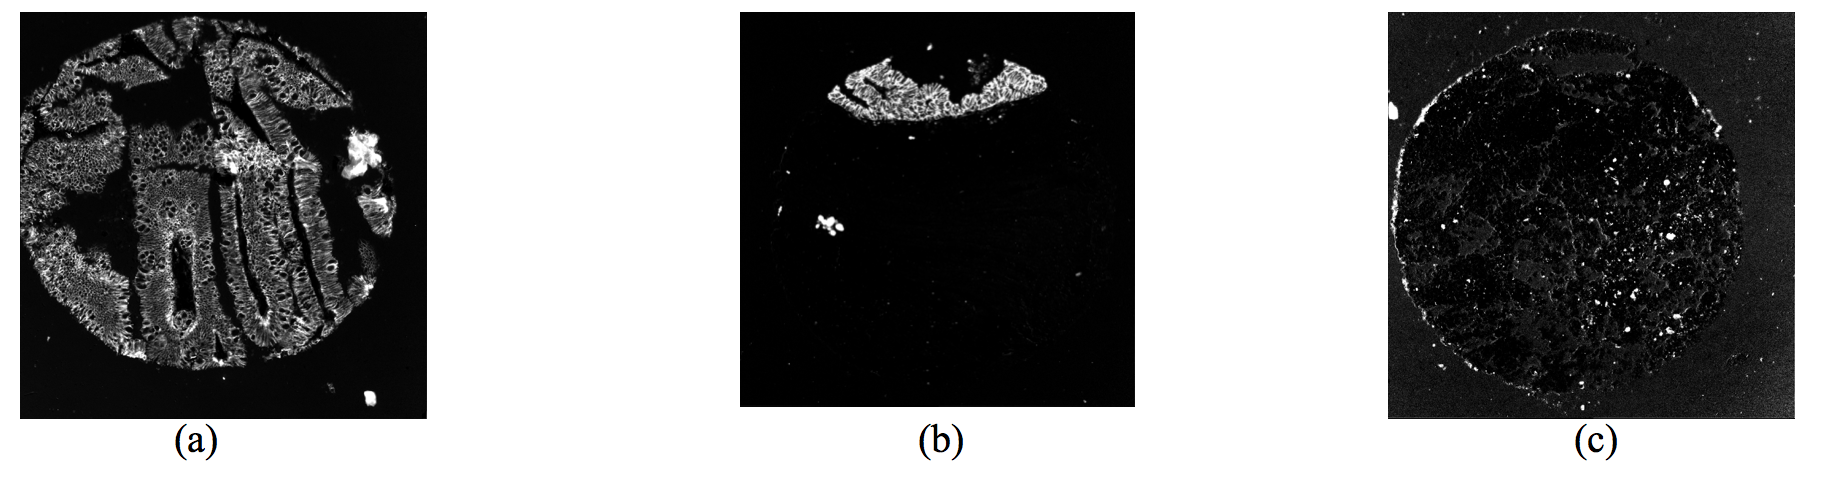
\includegraphics[width=1.0\textwidth]{img/ugly_samples}
\caption{Three sample images from E\_cad stained tissues}
\label{fig:ugly_samples}
\end{figure}

 \begin{figure}[H]
\centering
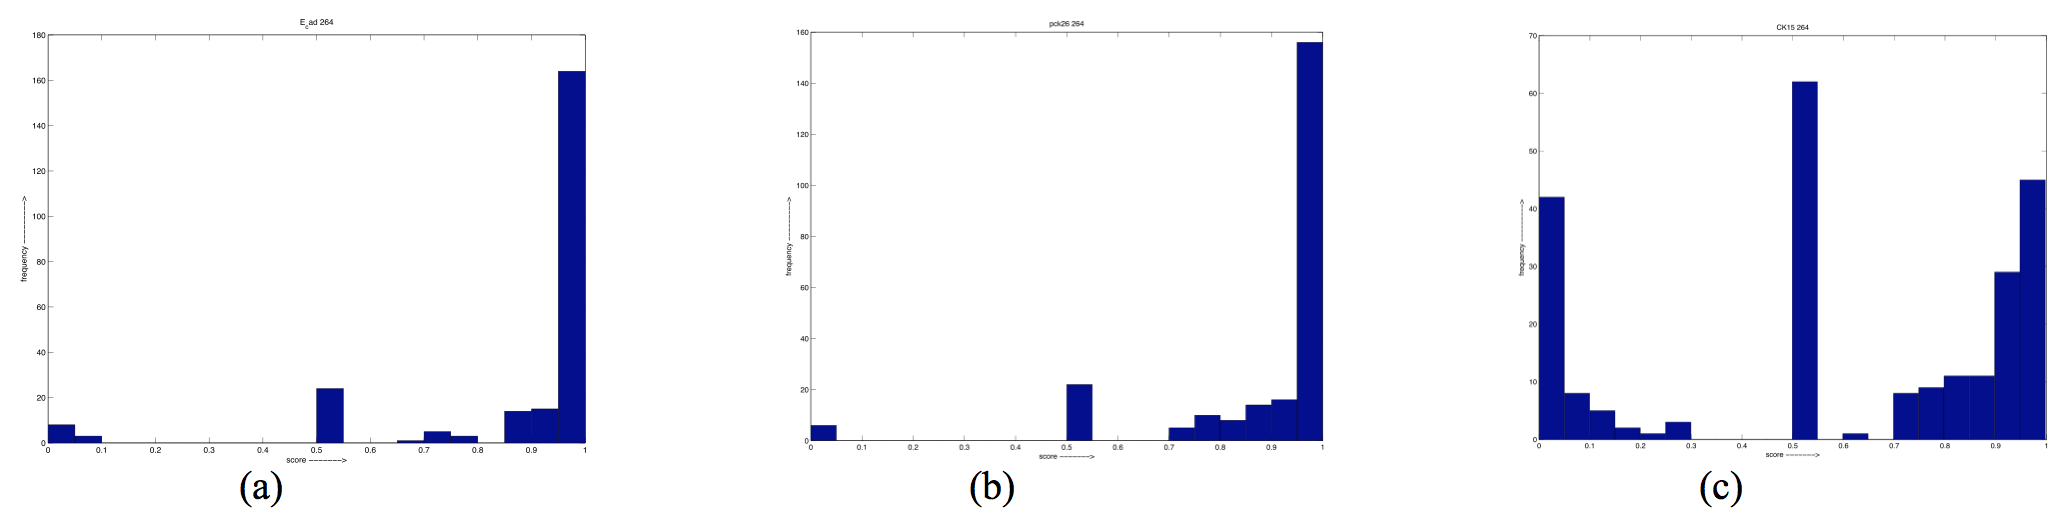
\includegraphics[width=1.0\textwidth]{img/ugly_distributions}
\caption{Discrete distributions of QoI scores for (a) E\_cad (b) pck26 (c) CK15}
\label{fig:ugly_distributions}
\end{figure}

\section{Conclusions}
We introduce in this paper a novel way to combine SVM and Naïve Bayes classifiers to form an image quality score.  The score is based on the confidence of a data point with respect to the classifier margin; and the distribution of the data captured by the Naïve Bayes classifier. Images that have high or low information content are easy to label as good or bad respectively. A labeling of the ugly class becomes dependent on the observer. Therefore computing a score is a more natural way of extracting this third class of images. The score helps us retrieve images that may have been discarded by a simple binary classification; or may have gone unnoticed by a human eye. Also, we use image analysis techniques to form a combined image that tries to capture the signal from all three markers.

